\documentclass{homework}

\usepackage{fixme}
\usepackage{graphicx}
\usepackage{hyperref}


\title{Practical Network Defense - Lab 9}
\subtitle{Vulnerability assessment of ACME co.'s network}
\author{Alessandro Serpi - 1647244}
\date{17 May 2019}


\begin{document}
    \maketitle
    \tableofcontents
    
    
    \pagebreak
    \section{Introduction}
    Vulnerability scanners are applicative designed to discover weaknesses in an environment, especially those caused by misconfigurations or flawed software components.
    Continuous vulnerability scanning is a staple of an effective cyberdefense policy.
    
    In this assignment we will execute a vulnerability scan of ACME co.'s private network.
    Then,  we will identify and apply fixes to the discovered weaknesses.
    If it will be not possible to completely resolve an issue, we will at least try to mitigate the vulnerability.
    
    
    \section{Greenbone setup}
    \subsection{Greenbone Community Edition in the local environment}
    Create a new VirtualBox virtual machine \textit{pnd-gsm}, selecting \textit{Linux} and \textit{Other Linux (64-bit)} as respectively OS type and version and assigning at least 4GiB of RAM and 9GiB of hard disk space.
    Then, download the latest ISO image of the Greenbone Community Edition and assign it to the CD interface of the virtual machine.
    
    Start the virtual machine with the attached configuration script \texttt{start\_vms.sh} using the parameter \texttt{gsm} and follow on-screen instructions to create a local and a web account.
    
    Since the firewalls must allow all traffic from and to the vulnerability scanner, we decided not to place the virtual machine in the \textit{DMZ} in order to not create holes in the firewall.
    Instead, we established it in the \textit{INTERNAL\_SERVERS} network, where it is more difficult for a potential attacker to exploit the firewalls' configuration.
    
    \subsection{Tasks}
    Login in the web GUI and create a new host in \textit{Assets} $\triangleright$ \textit{Hosts} for every machine in the network, filling \textit{Name} with the host's IP address and \textit{Comment} with a description.
    \vspace{-5pt}
    \begin{figure}[H]
        \centering
        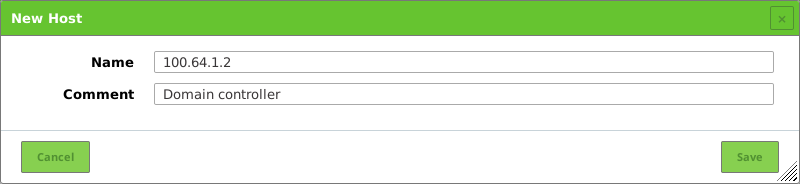
\includegraphics[width=1\linewidth]{images/new-host}
        \label{fig:new-host}
    \end{figure}
    \vspace{-20pt}
    
    Next, create new credentials in \textit{Configuration} $\triangleright$ \textit{Credentials} for every used SSH username/password combination.
    \vspace{-5pt}
    \begin{figure}[H]
        \centering
        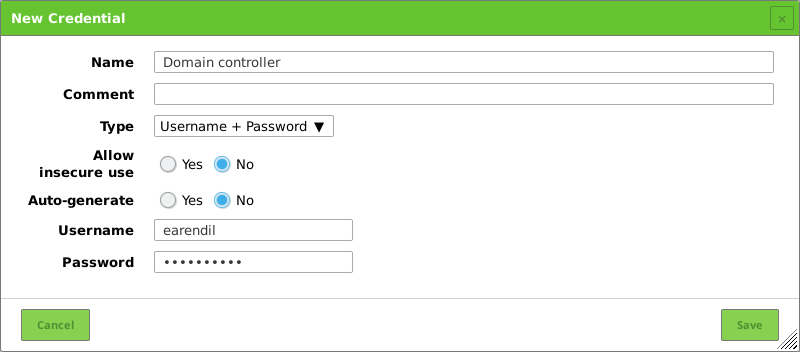
\includegraphics[width=1\linewidth]{images/new-credentials}
        \label{fig:new-credentials}
    \end{figure}
    \vspace{-20pt}
    
    In the host menu, create for each host a new target using the specific button.
    In the configuration window, select \textit{All IANA assigned TCP and UDP 2012-02-20} as \textit{Port List} and add the SSH credentials set (if it exists).
    
    Finally, in \textit{Scans} $\triangleright$ \textit{Tasks}, create a new task for every target, selecting \textit{Full and fast ultimate} as \textit{Scan Config} and \textit{Random} as \textit{Order for target hosts}.
    
    
    \section{Rules of engagement}
    We scanned all IANA-assigned TCP and UDP ports of every host in the private network.
    In addition, we gave to the vulnerability scanner SSH access to the resources in order to check for outdated and vulnerable components.
    
    Clients, log server and web server were analysed only in the remote environment, while (due to technical problems) the domain controller and the coffee maker were checked only in the local environment.
    Consequently, the mitigation described in section \hyperref[sec:http-mitigation]{5.1} was not implemented in the remote environment.
    
    
    \section{Assessment results and analysis}
    \subsection{Cleartext transmission of sensitive information via HTTP}
    \begin{displayquote}
        The host / application transmits sensitive information (username, passwords) in cleartext via HTTP.
        \textelp{}
        An attacker could use this situation to compromise or eavesdrop on the HTTP communication between the client and the server using a man-in-the-middle attack to get access to sensitive data like usernames or passwords.
    \end{displayquote}
    In order to allow ordinary and extraordinary maintenance, the coffee machine's web GUI must be accessible from the outside.
    Since communications between users and vending machine are carried out in cleartext using HTTP, an attacker that has access to the network can sniff user credentials or gain access to private data (such as the machine's current status).
    
    \subsection{Missing cookie attributes in the domain controller}
    \begin{displayquote}
        The application is missing the `httpOnly' attribute.
        \textelp{}
        This allows a cookie to be accessed by JavaScript which could lead to session hijacking attacks.
    \end{displayquote}
    \begin{displayquote}
        The flaw is due to cookie is not using 'secure' attribute, which allows cookie to be passed to the server by the client over non-secure channels (http) and allows attacker to conduct session hijacking attacks.
    \end{displayquote}
    The domain controller does not set `httpOnly' and `secure' cookie attributes, which can allow session hijacking attacks.
    Since this is a Zentyal's shortcoming, we can not implement any mitigation.
    
    \subsection{SSH brute force login with default credentials}
    \begin{displayquote}
        It was possible to login into the remote SSH server using default credentials.
       \textelp{}
       Change the password as soon as possible.
    \end{displayquote}
    In the remote environment, we left the default password for the majority of the resources.
    There were no such vulnerabilities in the local environment: when we created the servers, we chose non-default username/password combinations.
    
    \subsection{TCP timestamps}
    \begin{displayquote}
        It was detected that the host implements RFC1323.
        \textelp{}
        A side effect of this feature is that the uptime of the remote host can sometimes be computed.
    \end{displayquote}
    
    An attacker may use TCP timestamps to determine whether security patches requiring a reboot were applied to a host.
    However, disabling timestamps adds security through obscurity, which is no security. 
    In addition, TCP timestamps are used in the PAWS (Protect Against Wrapped Sequence Numbers) mechanism.
    
    Therefore, we decided not to consider the user of this functionality a vulnerability and not to implement any mitigation.
    
    
    \section{Mitigations}
    \subsection{Cleartext transmission of sensitive information via HTTP}\label{sec:http-mitigation}
    Since the vending machine does not support encryption, it is necessary to set up a TLS offloading mechanism to protect communications between the vending machine and the support crew.
    TLS operations are delegated to the main router, which encrypts messages coming from and decrypts messages directed to the vending machine. 
    
    Install \textit{os-nginx} in \textit{System} $\triangleright$ \textit{Firmware} $\triangleright$ \textit{Plugins}.
    Then, enable the web server in \textit{Services} $\triangleright$ \textit{Nginx} $\triangleright$ \textit{Configuration}.
    From now on all actions will be performed in \textit{nginx}'s configuration section.
    
    Create a new upstream server for the vending machine in \textit{Upstream} $\triangleright$ \textit{Upstream Server} and configure it like in the following image (leave all other fields unchanged), ensuring that \textit{Allow DNS server list to be overridden by DHCP/PPP on WAN } in \textit{System} $\triangleright$ \textit{Settings} $\triangleright$ \textit{General} is disabled.
    \vspace{-5pt}
    \begin{figure}[H]
        \centering
        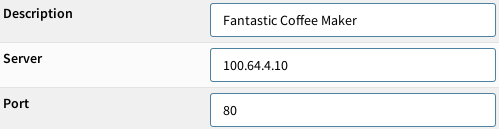
\includegraphics[width=\linewidth]{images/upstream-server}
        \label{fig:upstream-server}
    \end{figure}
    \vspace{-20pt}
    
    Create a new upstream in \textit{Upstream} $\triangleright$ \textit{Upstream} and configure it like in the following picture (leave all other fields unchanged).
    \vspace{-5pt}
    \begin{figure}[H]
        \centering
        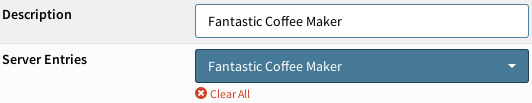
\includegraphics[width=1\linewidth]{images/upstream}
        \label{fig:upstream}
    \end{figure}
    \vspace{-20pt}
    
    Create a new location in \textit{HTTP(S)} $\triangleright$ \textit{Location} and configure it like in the following picture (leave all other fields unchanged).
    \vspace{-5pt}
    \begin{figure}[H]
        \centering
        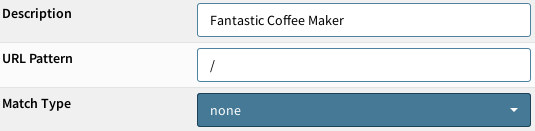
\includegraphics[width=1\linewidth]{images/location}
        \label{fig:location}
    \end{figure}
    \vspace{-20pt}
    
    Create a new certificate authority for the domain and a new server certificate for the subdomain \texttt{coffee-maker.pndeflab.edu}.
    
    Finally, create a new HTTP server in \textit{HTTP(S)} $\triangleright$ \textit{HTTP server} and configure it like in the following pictures (leave all other fields unchanged).
    It is especially important to select \textit{HTTPS Only}, otherwise users would still be able to carry on insecure communications with the server machine.
    \vspace{-5pt}
    \begin{figure}[H]
        \centering
        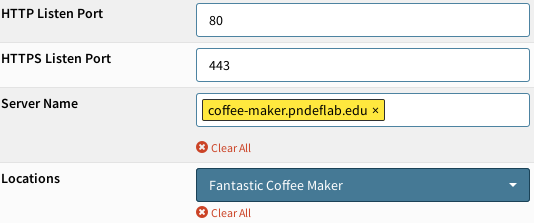
\includegraphics[width=1\linewidth]{images/http-server-1}
        \label{fig:http-server-1}
    \end{figure}
    \vspace{-20pt}
    \begin{figure}[H]
        \centering
        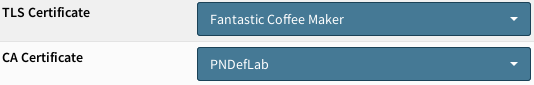
\includegraphics[width=1\linewidth]{images/http-server-2}
        \label{fig:http-server-2}
    \end{figure}
    \vspace{-20pt}
    \begin{figure}[H]
        \centering
        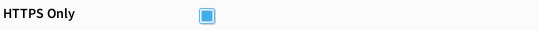
\includegraphics[width=1\linewidth]{images/http-server-3}
        \label{fig:http-server-3}
    \end{figure}
    \vspace{-20pt}
    
    Even if ACME's web server does not receive or transmit sensible information, we nonetheless decided to secure it in the same way performing analogous steps.
    
    \subsection{SSH brute force login with default credentials}
    Use non-predictable passwords also in the remote environment.
    
    
    \section{Final remarks}
    Overall, we found no serious security holes in the local environment directly ascribable to our actions (or inaction): all machines were properly configured and up to date.
    On the other hand, in the remote environment we deliberately chose not to change the default passwords in order to ease third-party checks, diminishing the security of the network.
\end{document}
